\documentclass[11pt]{article}
%\usepackage[utf8]{inputenc}

\usepackage{UCLAhandout_aditya}
\usepackage{course}
%%%%% NEW MATH DEFINITIONS %%%%%

\usepackage{amsmath,amsfonts,bm}

% Mark sections of captions for referring to divisions of figures
\newcommand{\figleft}{{\em (Left)}}
\newcommand{\figcenter}{{\em (Center)}}
\newcommand{\figright}{{\em (Right)}}
\newcommand{\figtop}{{\em (Top)}}
\newcommand{\figbottom}{{\em (Bottom)}}
\newcommand{\captiona}{{\em (a)}}
\newcommand{\captionb}{{\em (b)}}
\newcommand{\captionc}{{\em (c)}}
\newcommand{\captiond}{{\em (d)}}

% Highlight a newly defined term
\newcommand{\newterm}[1]{{\bf #1}}


% Figure reference, lower-case.
\def\figref#1{figure~\ref{#1}}
% Figure reference, capital. For start of sentence
\def\Figref#1{Figure~\ref{#1}}
\def\twofigref#1#2{figures \ref{#1} and \ref{#2}}
\def\quadfigref#1#2#3#4{figures \ref{#1}, \ref{#2}, \ref{#3} and \ref{#4}}
% Section reference, lower-case.
\def\secref#1{section~\ref{#1}}
% Section reference, capital.
\def\Secref#1{Section~\ref{#1}}
% Reference to two sections.
\def\twosecrefs#1#2{sections \ref{#1} and \ref{#2}}
% Reference to three sections.
\def\secrefs#1#2#3{sections \ref{#1}, \ref{#2} and \ref{#3}}
% Reference to an equation, lower-case.
% \def\eqref#1{equation~\ref{#1}}
% Reference to an equation, upper case
\def\Eqref#1{Equation~\ref{#1}}
% A raw reference to an equation---avoid using if possible
\def\plaineqref#1{\ref{#1}}
% Reference to a chapter, lower-case.
\def\chapref#1{chapter~\ref{#1}}
% Reference to an equation, upper case.
\def\Chapref#1{Chapter~\ref{#1}}
% Reference to a range of chapters
\def\rangechapref#1#2{chapters\ref{#1}--\ref{#2}}
% Reference to an algorithm, lower-case.
\def\algref#1{algorithm~\ref{#1}}
% Reference to an algorithm, upper case.
\def\Algref#1{Algorithm~\ref{#1}}
\def\twoalgref#1#2{algorithms \ref{#1} and \ref{#2}}
\def\Twoalgref#1#2{Algorithms \ref{#1} and \ref{#2}}
% Reference to a part, lower case
\def\partref#1{part~\ref{#1}}
% Reference to a part, upper case
\def\Partref#1{Part~\ref{#1}}
\def\twopartref#1#2{parts \ref{#1} and \ref{#2}}

\def\ceil#1{\lceil #1 \rceil}
\def\floor#1{\lfloor #1 \rfloor}
\def\1{\bm{1}}
\newcommand{\train}{D_{\mathrm{train}}}
\newcommand{\valid}{D_{\mathrm{valid}}}
\newcommand{\test}{D_{\mathrm{test}}}

% \newcommand{\train}{\mathcal{D}}
% \newcommand{\valid}{\mathcal{D_{\mathrm{valid}}}}
% \newcommand{\test}{\mathcal{D_{\mathrm{test}}}}

\def\eps{{\epsilon}}
\def\fid{{\textnormal{FID}}}


\def\calX{{\mathcal{X}}}
\def\calY{{\mathcal{Y}}}
\def\calZ{{\mathcal{Z}}}
\def\gxy{G_{\mathcal{X} \rightarrow  \mathcal{Y}}}
\def\gyx{G_{\mathcal{Y} \rightarrow  \mathcal{X}}}
\def\gzx{G_{\mathcal{Z} \rightarrow  \mathcal{X}}}
\def\gxz{G_{\mathcal{X} \rightarrow  \mathcal{Z}}}
\def\gzy{G_{\mathcal{Z} \rightarrow  \mathcal{Y}}}
\def\gyz{G_{\mathcal{Y} \rightarrow  \mathcal{Z}}}

% Random variables
% \def\reta{{\textnormal{$\eta$}}}
% \def\ra{{\textnormal{a}}}
% \def\rb{{\textnormal{b}}}
% \def\rc{{\textnormal{c}}}
% \def\rd{{\textnormal{d}}}
% \def\re{{\textnormal{e}}}
% \def\rf{{\textnormal{f}}}
% \def\rg{{\textnormal{g}}}
% \def\rh{{\textnormal{h}}}
% \def\ri{{\textnormal{i}}}
% \def\rj{{\textnormal{j}}}
% \def\rk{{\textnormal{k}}}
% \def\rl{{\textnormal{l}}}
% % rm is already a command, just don't name any random variables m
% \def\rn{{\textnormal{n}}}
% \def\ro{{\textnormal{o}}}
% \def\rp{{\textnormal{p}}}
% \def\rq{{\textnormal{q}}}
% \def\rr{{\textnormal{r}}}
% \def\rs{{\textnormal{s}}}
% \def\rt{{\textnormal{t}}}
% \def\ru{{\textnormal{u}}}
% \def\rv{{\textnormal{v}}}
% \def\rw{{\textnormal{w}}}
% \def\rx{{\textnormal{x}}}
% \def\ry{{\textnormal{y}}}
% \def\rz{{\textnormal{z}}}

\def\rx{{\textnormal{X}}}
\def\ry{{\textnormal{Y}}}
\def\rz{{\textnormal{Z}}}

% Random vectors
% \def\rvepsilon{{\mathbf{\epsilon}}}
% \def\rvtheta{{\mathbf{\theta}}}
% \def\rva{{\mathbf{a}}}
% \def\rvb{{\mathbf{b}}}
% \def\rvc{{\mathbf{c}}}
% \def\rvd{{\mathbf{d}}}
% \def\rve{{\mathbf{e}}}
% \def\rvf{{\mathbf{f}}}
% \def\rvg{{\mathbf{g}}}
% \def\rvh{{\mathbf{h}}}
% \def\rvu{{\mathbf{i}}}
% \def\rvj{{\mathbf{j}}}
% \def\rvk{{\mathbf{k}}}
% \def\rvl{{\mathbf{l}}}
% \def\rvm{{\mathbf{m}}}
% \def\rvn{{\mathbf{n}}}
% \def\rvo{{\mathbf{o}}}
% \def\rvp{{\mathbf{p}}}
% \def\rvq{{\mathbf{q}}}
% \def\rvr{{\mathbf{r}}}
% \def\rvs{{\mathbf{s}}}
% \def\rvt{{\mathbf{t}}}
% \def\rvu{{\mathbf{u}}}
% \def\rvv{{\mathbf{v}}}
% \def\rvw{{\mathbf{w}}}
% \def\rvx{{\mathbf{x}}}
% \def\rvy{{\mathbf{y}}}
% \def\rvz{{\mathbf{z}}}

\def\rvx{{\mathbf{X}}}
\def\rvy{{\mathbf{Y}}}
\def\rvz{{\mathbf{Z}}}

% Elements of random vectors
\def\erva{{\textnormal{a}}}
\def\ervb{{\textnormal{b}}}
\def\ervc{{\textnormal{c}}}
\def\ervd{{\textnormal{d}}}
\def\erve{{\textnormal{e}}}
\def\ervf{{\textnormal{f}}}
\def\ervg{{\textnormal{g}}}
\def\ervh{{\textnormal{h}}}
\def\ervi{{\textnormal{i}}}
\def\ervj{{\textnormal{j}}}
\def\ervk{{\textnormal{k}}}
\def\ervl{{\textnormal{l}}}
\def\ervm{{\textnormal{m}}}
\def\ervn{{\textnormal{n}}}
\def\ervo{{\textnormal{o}}}
\def\ervp{{\textnormal{p}}}
\def\ervq{{\textnormal{q}}}
\def\ervr{{\textnormal{r}}}
\def\ervs{{\textnormal{s}}}
\def\ervt{{\textnormal{t}}}
\def\ervu{{\textnormal{u}}}
\def\ervv{{\textnormal{v}}}
\def\ervw{{\textnormal{w}}}
\def\ervx{{\textnormal{x}}}
\def\ervy{{\textnormal{y}}}
\def\ervz{{\textnormal{z}}}

% Random matrices
\def\rmA{{\mathbf{A}}}
\def\rmB{{\mathbf{B}}}
\def\rmC{{\mathbf{C}}}
\def\rmD{{\mathbf{D}}}
\def\rmE{{\mathbf{E}}}
\def\rmF{{\mathbf{F}}}
\def\rmG{{\mathbf{G}}}
\def\rmH{{\mathbf{H}}}
\def\rmI{{\mathbf{I}}}
\def\rmJ{{\mathbf{J}}}
\def\rmK{{\mathbf{K}}}
\def\rmL{{\mathbf{L}}}
\def\rmM{{\mathbf{M}}}
\def\rmN{{\mathbf{N}}}
\def\rmO{{\mathbf{O}}}
\def\rmP{{\mathbf{P}}}
\def\rmQ{{\mathbf{Q}}}
\def\rmR{{\mathbf{R}}}
\def\rmS{{\mathbf{S}}}
\def\rmT{{\mathbf{T}}}
\def\rmU{{\mathbf{U}}}
\def\rmV{{\mathbf{V}}}
\def\rmW{{\mathbf{W}}}
\def\rmX{{\mathbf{X}}}
\def\rmY{{\mathbf{Y}}}
\def\rmZ{{\mathbf{Z}}}

% Elements of random matrices
\def\ermA{{\textnormal{A}}}
\def\ermB{{\textnormal{B}}}
\def\ermC{{\textnormal{C}}}
\def\ermD{{\textnormal{D}}}
\def\ermE{{\textnormal{E}}}
\def\ermF{{\textnormal{F}}}
\def\ermG{{\textnormal{G}}}
\def\ermH{{\textnormal{H}}}
\def\ermI{{\textnormal{I}}}
\def\ermJ{{\textnormal{J}}}
\def\ermK{{\textnormal{K}}}
\def\ermL{{\textnormal{L}}}
\def\ermM{{\textnormal{M}}}
\def\ermN{{\textnormal{N}}}
\def\ermO{{\textnormal{O}}}
\def\ermP{{\textnormal{P}}}
\def\ermQ{{\textnormal{Q}}}
\def\ermR{{\textnormal{R}}}
\def\ermS{{\textnormal{S}}}
\def\ermT{{\textnormal{T}}}
\def\ermU{{\textnormal{U}}}
\def\ermV{{\textnormal{V}}}
\def\ermW{{\textnormal{W}}}
\def\ermX{{\textnormal{X}}}
\def\ermY{{\textnormal{Y}}}
\def\ermZ{{\textnormal{Z}}}

% Vectors
% \def\vzero{{\bm{0}}}
% \def\vone{{\bm{1}}}
% \def\vmu{{\bm{\mu}}}
% \def\vtheta{{\bm{\theta}}}
% \def\va{{\bm{a}}}
% \def\vb{{\bm{b}}}
% \def\vc{{\bm{c}}}
% \def\vd{{\bm{d}}}
% \def\ve{{\bm{e}}}
% \def\vf{{\bm{f}}}
% \def\vg{{\bm{g}}}
% \def\vh{{\bm{h}}}
% \def\vi{{\bm{i}}}
% \def\vj{{\bm{j}}}
% \def\vk{{\bm{k}}}
% \def\vl{{\bm{l}}}
% \def\vm{{\bm{m}}}
% \def\vn{{\bm{n}}}
% \def\vo{{\bm{o}}}
% \def\vp{{\bm{p}}}
% \def\vq{{\bm{q}}}
% \def\vr{{\bm{r}}}
% \def\vs{{\bm{s}}}
% \def\vt{{\bm{t}}}
% \def\vu{{\bm{u}}}
% \def\vv{{\bm{v}}}
% \def\vw{{\bm{w}}}
% \def\vx{{\bm{x}}}
% \def\vy{{\bm{y}}}
% \def\vz{{\bm{z}}}
\def\va{{\mathbf{a}}}
\def\vs{{\mathbf{s}}}
\def\vx{{\mathbf{x}}}
\def\vy{{\mathbf{y}}}
\def\vz{{\mathbf{z}}}

% Elements of vectors
\def\evalpha{{\alpha}}
\def\evbeta{{\beta}}
\def\evepsilon{{\epsilon}}
\def\evlambda{{\lambda}}
\def\evomega{{\omega}}
\def\evmu{{\mu}}
\def\evpsi{{\psi}}
\def\evsigma{{\sigma}}
\def\evtheta{{\theta}}
\def\eva{{a}}
\def\evb{{b}}
\def\evc{{c}}
\def\evd{{d}}
\def\eve{{e}}
\def\evf{{f}}
\def\evg{{g}}
\def\evh{{h}}
\def\evi{{i}}
\def\evj{{j}}
\def\evk{{k}}
\def\evl{{l}}
\def\evm{{m}}
\def\evn{{n}}
\def\evo{{o}}
\def\evp{{p}}
\def\evq{{q}}
\def\evr{{r}}
\def\evs{{s}}
\def\evt{{t}}
\def\evu{{u}}
\def\evv{{v}}
\def\evw{{w}}
\def\evx{{x}}
\def\evy{{y}}
\def\evz{{z}}

% Matrix
\def\mA{{\bm{A}}}
\def\mB{{\bm{B}}}
\def\mC{{\bm{C}}}
\def\mD{{\bm{D}}}
\def\mE{{\bm{E}}}
\def\mF{{\bm{F}}}
\def\mG{{\bm{G}}}
\def\mH{{\bm{H}}}
\def\mI{{\bm{I}}}
\def\mJ{{\bm{J}}}
\def\mK{{\bm{K}}}
\def\mL{{\bm{L}}}
\def\mM{{\bm{M}}}
\def\mN{{\bm{N}}}
\def\mO{{\bm{O}}}
\def\mP{{\bm{P}}}
\def\mQ{{\bm{Q}}}
\def\mR{{\bm{R}}}
\def\mS{{\bm{S}}}
\def\mT{{\bm{T}}}
\def\mU{{\bm{U}}}
\def\mV{{\bm{V}}}
\def\mW{{\bm{W}}}
\def\mX{{\bm{X}}}
\def\mY{{\bm{Y}}}
\def\mZ{{\bm{Z}}}
\def\mBeta{{\bm{\beta}}}
\def\mPhi{{\bm{\Phi}}}
\def\mLambda{{\bm{\Lambda}}}
\def\mSigma{{\bm{\Sigma}}}

% Tensor
\DeclareMathAlphabet{\mathsfit}{\encodingdefault}{\sfdefault}{m}{sl}
\SetMathAlphabet{\mathsfit}{bold}{\encodingdefault}{\sfdefault}{bx}{n}
\newcommand{\tens}[1]{\bm{\mathsfit{#1}}}
\def\tA{{\tens{A}}}
\def\tB{{\tens{B}}}
\def\tC{{\tens{C}}}
\def\tD{{\tens{D}}}
\def\tE{{\tens{E}}}
\def\tF{{\tens{F}}}
\def\tG{{\tens{G}}}
\def\tH{{\tens{H}}}
\def\tI{{\tens{I}}}
\def\tJ{{\tens{J}}}
\def\tK{{\tens{K}}}
\def\tL{{\tens{L}}}
\def\tM{{\tens{M}}}
\def\tN{{\tens{N}}}
\def\tO{{\tens{O}}}
\def\tP{{\tens{P}}}
\def\tQ{{\tens{Q}}}
\def\tR{{\tens{R}}}
\def\tS{{\tens{S}}}
\def\tT{{\tens{T}}}
\def\tU{{\tens{U}}}
\def\tV{{\tens{V}}}
\def\tW{{\tens{W}}}
\def\tX{{\tens{X}}}
\def\tY{{\tens{Y}}}
\def\tZ{{\tens{Z}}}


% Graph
\def\gA{{\mathcal{A}}}
\def\gB{{\mathcal{B}}}
\def\gC{{\mathcal{C}}}
\def\gD{{\mathcal{D}}}
\def\gE{{\mathcal{E}}}
\def\gF{{\mathcal{F}}}
\def\gG{{\mathcal{G}}}
\def\gH{{\mathcal{H}}}
\def\gI{{\mathcal{I}}}
\def\gJ{{\mathcal{J}}}
\def\gK{{\mathcal{K}}}
\def\gL{{\mathcal{L}}}
\def\gM{{\mathcal{M}}}
\def\gN{{\mathcal{N}}}
\def\gO{{\mathcal{O}}}
\def\gP{{\mathcal{P}}}
\def\gQ{{\mathcal{Q}}}
\def\gR{{\mathcal{R}}}
\def\gS{{\mathcal{S}}}
\def\gT{{\mathcal{T}}}
\def\gU{{\mathcal{U}}}
\def\gV{{\mathcal{V}}}
\def\gW{{\mathcal{W}}}
\def\gX{{\mathcal{X}}}
\def\gY{{\mathcal{Y}}}
\def\gZ{{\mathcal{Z}}}

% Sets
\def\sA{{\mathbb{A}}}
\def\sB{{\mathbb{B}}}
\def\sC{{\mathbb{C}}}
\def\sD{{\mathbb{D}}}
% Don't use a set called E, because this would be the same as our symbol
% for expectation.
\def\sF{{\mathbb{F}}}
\def\sG{{\mathbb{G}}}
\def\sH{{\mathbb{H}}}
\def\sI{{\mathbb{I}}}
\def\sJ{{\mathbb{J}}}
\def\sK{{\mathbb{K}}}
\def\sL{{\mathbb{L}}}
\def\sM{{\mathbb{M}}}
\def\sN{{\mathbb{N}}}
\def\sO{{\mathbb{O}}}
\def\sP{{\mathbb{P}}}
\def\sQ{{\mathbb{Q}}}
\def\sR{{\mathbb{R}}}
\def\sS{{\mathbb{S}}}
\def\sT{{\mathbb{T}}}
\def\sU{{\mathbb{U}}}
\def\sV{{\mathbb{V}}}
\def\sW{{\mathbb{W}}}
\def\sX{{\mathbb{X}}}
\def\sY{{\mathbb{Y}}}
\def\sZ{{\mathbb{Z}}}

% Entries of a matrix
\def\emLambda{{\Lambda}}
\def\emA{{A}}
\def\emB{{B}}
\def\emC{{C}}
\def\emD{{D}}
\def\emE{{E}}
\def\emF{{F}}
\def\emG{{G}}
\def\emH{{H}}
\def\emI{{I}}
\def\emJ{{J}}
\def\emK{{K}}
\def\emL{{L}}
\def\emM{{M}}
\def\emN{{N}}
\def\emO{{O}}
\def\emP{{P}}
\def\emQ{{Q}}
\def\emR{{R}}
\def\emS{{S}}
\def\emT{{T}}
\def\emU{{U}}
\def\emV{{V}}
\def\emW{{W}}
\def\emX{{X}}
\def\emY{{Y}}
\def\emZ{{Z}}
\def\emSigma{{\Sigma}}

% entries of a tensor
% Same font as tensor, without \bm wrapper
\newcommand{\etens}[1]{\mathsfit{#1}}
\def\etLambda{{\etens{\Lambda}}}
\def\etA{{\etens{A}}}
\def\etB{{\etens{B}}}
\def\etC{{\etens{C}}}
\def\etD{{\etens{D}}}
\def\etE{{\etens{E}}}
\def\etF{{\etens{F}}}
\def\etG{{\etens{G}}}
\def\etH{{\etens{H}}}
\def\etI{{\etens{I}}}
\def\etJ{{\etens{J}}}
\def\etK{{\etens{K}}}
\def\etL{{\etens{L}}}
\def\etM{{\etens{M}}}
\def\etN{{\etens{N}}}
\def\etO{{\etens{O}}}
\def\etP{{\etens{P}}}
\def\etQ{{\etens{Q}}}
\def\etR{{\etens{R}}}
\def\etS{{\etens{S}}}
\def\etT{{\etens{T}}}
\def\etU{{\etens{U}}}
\def\etV{{\etens{V}}}
\def\etW{{\etens{W}}}
\def\etX{{\etens{X}}}
\def\etY{{\etens{Y}}}
\def\etZ{{\etens{Z}}}

% The true underlying data generating distribution
\newcommand{\pdata}{p_{\rm{data}}}
% The empirical distribution defined by the training set
\newcommand{\ptrain}{\hat{p}_{\rm{data}}}
\newcommand{\Ptrain}{\hat{P}_{\rm{data}}}
% The model distribution
\newcommand{\ptheta}{p_{\theta}}
\newcommand{\Ptheta}{P_{\theta}}
\newcommand{\ptildemodel}{\tilde{p}_{\theta}}
% \newcommand{\pmodel}{p_{\rm{model}}}
% \newcommand{\Pmodel}{P_{\rm{model}}}
% \newcommand{\ptildemodel}{\tilde{p}_{\rm{model}}}
% Stochastic autoencoder distributions
\newcommand{\pencode}{p_{\rm{encoder}}}
\newcommand{\pdecode}{p_{\rm{decoder}}}
\newcommand{\precons}{p_{\rm{reconstruct}}}

\newcommand{\laplace}{\mathrm{Laplace}} % Laplace distribution

% \newcommand{\E}{\mathbb{E}}
\newcommand{\Ls}{\mathcal{L}}
% \newcommand{\R}{\mathbb{R}}
\newcommand{\emp}{\tilde{p}}
\newcommand{\lr}{\alpha}
\newcommand{\reg}{\lambda}
\newcommand{\rect}{\mathrm{rectifier}}
\newcommand{\softmax}{\mathrm{softmax}}
\newcommand{\sigmoid}{\sigma}
\newcommand{\softplus}{\zeta}
\newcommand{\KL}{D_{\mathrm{KL}}}
\newcommand{\Var}{\mathrm{Var}}
\newcommand{\standarderror}{\mathrm{SE}}
\newcommand{\Cov}{\mathrm{Cov}}
% Wolfram Mathworld says $L^2$ is for function spaces and $\ell^2$ is for vectors
% But then they seem to use $L^2$ for vectors throughout the site, and so does
% wikipedia.
\newcommand{\normlzero}{L^0}
\newcommand{\normlone}{L^1}
\newcommand{\normltwo}{L^2}
\newcommand{\normlp}{L^p}
\newcommand{\normmax}{L^\infty}

\newcommand{\parents}{Pa} % See usage in notation.tex. Chosen to match Daphne's book.

% \DeclareMathOperator*{\argmax}{arg\,max}
% \DeclareMathOperator*{\argmin}{arg\,min}

\DeclareMathOperator{\sign}{sign}
\DeclareMathOperator{\Tr}{Tr}
\let\ab\allowbreak


\usepackage{color,amssymb,stmaryrd,amsmath,amsfonts,rotating,mathrsfs,psfrag}
\usepackage{listings}

\newcommand{\ag}[1]{\textcolor{red}{[AG: #1]}}

\begin{document}

\solntrue

\handout{23th May 2023}{\Large Homework 4 \\ \small Due 6th June 2023, Tuesday, before 11:59 pm}
 
\newif\ifaditya
\adityatrue

\vspace{-0.5in}
\newtheorem{lemma}{Lemma}[section]

\exercise[Weighted PCA \problemworth{5}]
 Let $\vct{x}^{(1)},\ldots, \vct{x}^{(n)}$ be $n$ vectors in $\mathbb{R}^d$. We want to map these vectors into a lower dimensional space $\mathbb{R}^m$ where $m < d$, and then be able to recover the vectors from their lower dimensional representation. PCA finds matrices $W\in\mathbb{R}^{m\times d}$ and $U\in\mathbb{R}^{d\times m}$ such that $W$ maps $\vct{x}^{(i)}$ into a lower dimensional space; i.e., $\vct{y}^{(i)} = W\vct{x}^{(i)}$. And $U$ tries to recover $\vct{x}^{(i)}$ from $\vct{y}^{(i)}$; i.e., $\tilde{\vct{x}}^{(i)} = U\vct{y}^{(i)} = UW\vct{x}^{(i)}$. In PCA, we want to solve: 
 \begin{equation}
 \label{eq: pca}
     \min_{W\in\mathbb{R}^{m\times d}, U\in\mathbb{R}^{d\times m}} \sum_{i=1}^{n} \left\lVert  \vct{x}^{(i)} - UW\vct{x}^{(i)}\right\rVert_2^2.
 \end{equation}
As shown in the class, the solution for this problem is given by the following lemmas:
\begin{lemma}
The problem \eqref{eq: pca} can be recast as: 
\begin{equation}
    \min_{ U\in\mathbb{R}^{d\times m}, U^TU = I_m} \sum_{i=1}^{n} \left\lVert  \vct{x}^{(i)} - UU^T\vct{x}^{(i)}\right\rVert_2^2.
\end{equation}
In other words, the solution for this problem is to find a $W = U^T$ for some $U$ such that $U^TU = I_m$.
\end{lemma}
 
\paragraph{Weighted PCA} Now, suppose we change the objective function of PCA to:
\[
\mathop{\text{min}}_{W\in\mathbb{R}^{m\times d}, U\in\mathbb{R}^{d\times m}}\sum^n_{i=1}\gamma_i\|\mathbf{x}^{(i)}-\widetilde{\mathbf{x}}^{(i)}\|^2_2
\]
where $\gamma_i>0$ and $\tilde{\vct{x}}^{(i)} = UW\vct{x}^{(i)}$, $\forall i$. 
Prove that the objective function can be recast as
  \[
     \mathop{\text{min}}_{U\in\mathbb{R}^{d\times m}, U^TU = I_{m}}\sum^n_{i=1}\gamma_i \|\mathbf{x}^{(i)}-UU^T{\mathbf{x}^{(i)}}\|^2_2.
\]
[\textbf{Hint:} You can directly use Lemma 1 (without proof) as a subroutine in your overall proof].

\newpage \
 \vspace{5cm} \
\exercise[A Two-Layer Neural Network for Binary Classification \problemworth{12}]
In this exercise, we will walk through the forward and backward propagation process for a two-layer fully connected neural network. We will use the same data as in Homework 1, the MNIST dataset. The data you will be using is under the \verb|MNIST| folder.

\begin{enumerate}
    \item \itemworth{0} Load and visualize the data by running the cells for Part (a) in the notebook.   
    
    \item \itemworth{2} Implement the forward pass of the two-layer feed forward neural network with a ReLU non-linear layer. Specifically, implement code of ``part (b)'' to compute \verb|scores| in the \verb|loss()| function, take a screenshot of your code and paste it here. Further information and guidance are provided in the comments of the code.\\
    (\emph{Hint}: Our network has four set of parameters to be updated: First layer weights, first layer biases, second layer weights, and second layer biases. The weights and bias parameters are initialized in the \verb|__init__()| function of the \verb|TwoLayerNet| class.)
    \vspace{4cm}
    
    \item \itemworth{1} What is the formula for calculating $\ell_2$ regularization? Write it down here. Implement the $\ell_2$ regularization term in ``part (c)'', take a screenshot of your code and paste it here. \\
    \vspace{4cm}
    
    \item \itemworth{2} Recall that we can express the final hypothesis for a binary classifier using sigmoid (only 1 output unit) or softmax (2 output units). Implement the softmax cross entropy loss and the gradient w.r.t the inputs in the function \verb|softmax_loss(x,y)|, take a screenshot of your code and paste it here.\\
    Suppose your softmax cross entropy loss function takes $\boldsymbol{X}$ and  $\boldsymbol{Y}$ as inputs. Specifically, input $\boldsymbol{X}$ is the output score after the second layer, where $x^{(i)}_j$ is the output score of sample $i$ being in class $j$; input $\boldsymbol{Y}$ is the target label represented as one-hot vectors, where $y^{(i)}\in\mathbb{R}^C$ is the one-hot encoded label of sample $i$, e.g, for binary classification,  $y^{(i)} = \left[0, 1\right]$ or $y^{(i)} = \left[1, 0\right]$. What is the formula for calculating the softmax cross-entropy loss and gradient? Write it down here. You can write your formula using $x^{(i)}_j$ and $y^{(i)}_j$.\\
    \vspace{4cm}

    \item \itemworth{3} Implement the back-propagation process by completing the gradient computation for W2 and b2 in ``part (e)'', take a screenshot of your code and paste it here. What is the formula for calculating the gradient of W2 and b2? Write it down here.\\
    \vspace{4cm}

    \item \itemworth{4} Implement the prediction function in ``part (f)'' and check the correctness of your implementation above by running the predictions on validation and test sets. Adjust the learning rate in $10^{-5}, 10^{-4}, 10^{-3}, 5\times10^{-3}, 10^{-1}$. Report the best accuracy you get and the corresponding learning rate. Briefly discuss your observations of using different learning rates.\\
    \vspace{4cm}

\end{enumerate}



\exercise[K-Means Clustering \problemworth{15}]

In this problem, we shall apply K-Means Algorithm to a popular visual classification dataset CIFAR-10 \footnote{\url{https://www.cs.toronto.edu/~kriz/cifar.html}}. CIFAR-10 dataset consists of 60K labeled 32 x 32 colored images i.e., each image would have 3 channels corresponding to RGB colors.
Out of the total 60K images, 50K images belong to the training set and 10K belong to the testing set. Within the scope of this problem, we shall work with the testing set only for computational efficiency purposes. Additionally, as K-Means is an unsupervised learning algorithm, we shall discard the labels associated with the images.

Please find the code skeleton for this problem in \verb|Sp23-CS146-HW4.ipynb| notebook shared with you as a part of this HW.

\subsection*{A Implementing K-Means}
 Rather than training K-Means from scratch, we are going to make use of a pre-existing implementation available in scikit-learn.\footnote{\url{https://scikit-learn.org/stable/modules/generated/sklearn.cluster.KMeans.html}}

\begin{enumerate}
\item \itemworth{5} Make use of the \verb|dataloader()| function to load the data in our notebook. Within this function, the data is loaded using \verb|datasets| package in Tensorflow. \footnote{\url{https://www.tensorflow.org/datasets/catalog/cifar10#:~:text=The\%20CIFAR\%2D10\%20dataset\%20consists,images\%20and\%2010000\%20test\%20images.\&text=Versions\%3A,3.0.}} \textbf{Tip}: Run this notebook in Google Colab as it saves you a lot of time spent in installing Tensorflow.

This function will return 10K testing images of CIFAR-10 dataset along with their ground truth label. We provide \verb|visualize(X, ind)| function to visualize index \verb|ind| in the data \verb|X|. Before using K-Means algorithm, we need to make that the data is as 10000 N-dimensional vector instead of (10000, 32, 32, 3) tensor. Your first task would be to implement \verb|reshape| function that will convert the tensor form of the input to a 2D matrix of the form 10000 x N where N = 32 x 32 x 3. Take a screenshot of your code and paste it here. \hfill 
\vspace{4cm}

\item \itemworth{5} Once you have reshaped your input, you are ready to apply K-Means algorithm to your data. Note that the number of cluster centers K is a hyperparameter. As we are in the unsupervised regime, we do not have access to any labeled validation set that could be used to decide the best for K. Thus, we use some pre-defined metrics to decide what choice of K should be the best. In this HW, we are going to use the \textit{Sum of squared distances of samples to their closest cluster center} as our score metric. However, we are also aware that K-Means algorithm can lead to different convergence based on the initialization of the clusters. To account for the differences between the score due to various initializations, we apply the algorithm across 3 random seeds (\verb|random_state| in the code). Here, your task is to write a few lines of code to fit the K-Means algorithm and calculate the score metric for all three runs, take a screenshot of your code and paste it here. Finally, submit the results graph you get after running the plotting block in the notebook that takes in your calculated scores as the input.\hfill 
\vspace{5cm}
\end{enumerate}

\subsection*{B Visualization} \itemworth{5}
Another aspect of applying K-Means algorithm involves visualizing the cluster assignments. As described above, the CIFAR-10 data is 3092 dimensional (32 x 32 x 3) which is quite impossible to visualize for us. However, we can project our high dimensional input data into lower dimensional space using PCA algorithm discussed in the class. Once you have the PCA output of the data, we can visualize the transformed low dimensional data easily.

We provide a simple implementation of PCA using its support in \verb|sklearn.decomposition|. To get some sense of how PCA can be beneficial in plotting the high dimensional data, we provide a code block that provides you the PCA of the input data along with its ground truth labels. Running that block should output a plot which looks like Figure \ref{fig:my_label}. 

\begin{figure}[h]
    \centering
    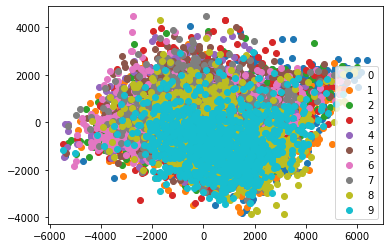
\includegraphics[scale=0.7]{figs/pca-cifar10.png}
    \caption{PCA of CIFAR-10 test data in 2-D with ground truth labels.}
    \label{fig:my_label}
\end{figure}

Your task is to first apply K-means algorithm with K = 10 and \verb|random_state = 42| to the input data, and get the predicted label assignments to each data sample. Careful inspection of the K-Means documentation should help you to get the predicted labels in one-line of code. Using these predicted labels, implement a code to get a scatter plot of the low-dimensional PCA data with these new assignments. Take a screenshot of your code and paste it here. Submit the final graph you get for this part. \hfill

\end{document}
